See Fig. \ref{fig:3.12.6_tri_1}.  Let $AB$ be the base and $\vec{M}$ be the midpoint.
Then, 
\begin{align}
\vec{A} = \myvec{0\\a},
\vec{B} = \myvec{0\\-a}
\end{align}
If 
\begin{align}
\vec{C} &= \myvec{p\\0}, 
\\
\norm{\vec{C}-\vec{A}} &= 2a
\implies 
\sqrt{p^2+a^2} &= 2a
\\
\text{or, } p = \pm\sqrt{3}a
\end{align}
resulting in two possible triangles as in Fig. \ref{fig:3.12.6_tri_1}.
%
$\triangle{ABC}$ in Fig.\ref{fig:3.12.6_tri_1}  is generated using the following python code
\begin{lstlisting}
solutions/6/codes/line/miscellaneous/tri_equi.py
\end{lstlisting}
\begin{figure}[!ht]
\centering
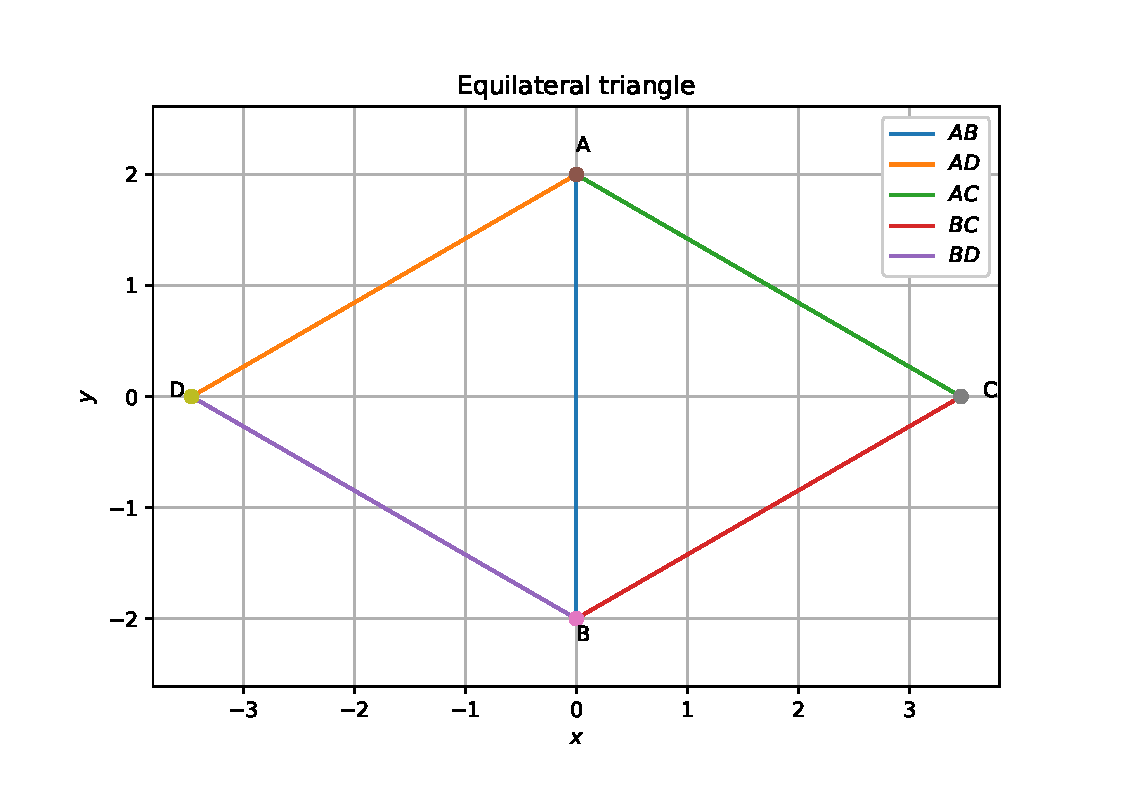
\includegraphics[width=\columnwidth]{./solutions/6/codes/line/miscellaneous/tri_equi.eps}
\caption{Triangles $ABC$ and $ABD$ using python}
\label{fig:3.12.6_tri_1}
\end{figure} 


